\documentclass[12pt, a4paper]{article}

% 패키지
\usepackage[utf8]{inputenc}
\usepackage[T1]{fontenc}
\usepackage{kotex}
\usepackage{graphicx}
\usepackage{booktabs}
\usepackage{caption}
\usepackage{subcaption}
\usepackage{geometry}
\usepackage{amsmath}
\usepackage{hyperref}
\usepackage{float}
\usepackage{xcolor}
\usepackage{tocloft}
\usepackage{titlesec}
\usepackage{fancyvrb}

% 페이지 설정
\geometry{margin=2.5cm}

% 색상 정의
\definecolor{primary}{HTML}{2C3E50}
\definecolor{accent}{HTML}{3498DB}

% 제목 스타일
\titleformat{\section}{\Large\bfseries\color{primary}}{\thesection}{1em}{}
\titleformat{\subsection}{\large\bfseries\color{primary}}{\thesubsection}{1em}{}

% APA 스타일 캡션
\captionsetup{
    format=plain,
    labelfont=bf,
    font=small,
    labelsep=newline,
    justification=raggedright,
    singlelinecheck=false
}

\begin{document}

% 표지
\begin{titlepage}
    \centering
    \vspace*{3cm}
    {\Huge\bfseries\color{primary} EmpathyAI 프로젝트 보고서\par}
    \vspace{1cm}
    {\Large 공감 수준 분류를 위한 LLM Fine-tuning\par}
    \vspace{2cm}
    {\large OPELA 데이터셋 기반 GPT-4.1 Nano 모델 최적화\par}
    \vspace{3cm}
    {\large \today\par}
    \vfill
    {\normalsize Smilegate AI \& 서울대학교 공동 연구 데이터 활용\par}
\end{titlepage}

% 목차
\tableofcontents
\newpage

% ============================================
% 1. 서론
% ============================================
\section{서론}

\subsection{연구 배경}
대화형 AI 시스템에서 공감 능력은 사용자 경험의 핵심 요소이다. 
본 프로젝트는 한국어 대화에서 AI(페르소나)의 공감 수준을 자동으로 분류하는 시스템을 개발하였다.
OPELA(Open-domain conversations by Personas with Empathy, Long-term memory, and Attractive personality) 
데이터셋을 활용하여 GPT-4.1 Nano 모델을 fine-tuning하였다.

\subsection{연구 목표}
\begin{itemize}
    \item 한국어 페르소나-유저 대화에서 공감 수준 자동 분류
    \item 5단계 공감 레벨(0-4) 분류 모델 개발
    \item Base 모델 대비 Fine-tuned 모델 성능 향상 검증
\end{itemize}

\subsection{공감 레벨 정의}
본 연구에서 사용한 공감 레벨은 Table~\ref{tab:empathy_levels}과 같이 정의된다.

\begin{table}[H]
\centering
\caption{Empathy Level Definitions}
\label{tab:empathy_levels}
\begin{tabular}{clp{8cm}}
\toprule
\textbf{Level} & \textbf{Label} & \textbf{Description} \\
\midrule
0 & Not Applicable & 공감이 적용되지 않는 상황 (인사, 단순 정보 교환 등) \\
1 & Empathy Failure & 공감 실패 (상대방의 감정을 무시하거나 부적절한 반응) \\
2 & Low Empathy & 낮은 수준의 공감 (최소한의 반응만 제공) \\
3 & Moderate Empathy & 중간 수준의 공감 (적절한 감정적 반응) \\
4 & High Active Empathy & 높은 수준의 적극적 공감 (깊은 이해와 적극적 지지) \\
\bottomrule
\end{tabular}

\vspace{0.5em}
\footnotesize\textit{Note.} 공감 레벨은 제3자 평가자(labeler)에 의해 라벨링되었으며, 다수결 투표를 통해 최종 레이블이 결정되었다.
\end{table}

% ============================================
% 2. 데이터셋
% ============================================
\section{데이터셋}

\subsection{OPELA 데이터셋 개요}
OPELA 데이터셋은 Smilegate AI와 서울대학교의 공동 연구 프로젝트로 수집되었다.
실제 크라우드워커 간의 페르소나-유저 역할극 대화로 구성되어 있으며, 
15턴에서 80턴까지의 다양한 일상 주제를 포함한다.

\subsection{데이터 통계}
본 연구에서 사용한 데이터의 기술 통계는 Table~\ref{tab:data_stats}에 제시되어 있다.

\begin{table}[H]
\centering
\caption{Descriptive Statistics of the OPELA Dataset}
\label{tab:data_stats}
\begin{tabular}{lr}
\toprule
\textbf{Statistic} & \textbf{Value} \\
\midrule
Total Samples & 14,825 \\
Unique Conversations & 533 \\
Average Turns per Conversation & 30.14 \\
Average User Text Length (chars) & 48.03 \\
Average Persona Text Length (chars) & 45.53 \\
\bottomrule
\end{tabular}

\vspace{0.5em}
\footnotesize\textit{Note.} 텍스트 길이는 한글 문자 기준으로 측정되었다.
\end{table}

\subsection{라벨 분포}
전체 데이터셋의 공감 레벨 분포는 Table~\ref{tab:label_dist}와 Figure~\ref{fig:label_dist}에 제시되어 있다.

\begin{table}[H]
\centering
\caption{Empathy Label Distribution in the Full Dataset}
\label{tab:label_dist}
\begin{tabular}{crrr}
\toprule
\textbf{Label} & \textbf{Count} & \textbf{Percentage} & \textbf{Cumulative \%} \\
\midrule
0 & 4,167 & 28.1\% & 28.1\% \\
1 & 660 & 4.5\% & 32.6\% \\
2 & 1,806 & 12.2\% & 44.7\% \\
3 & 7,198 & 48.6\% & 93.3\% \\
4 & 994 & 6.7\% & 100.0\% \\
\midrule
\textbf{Total} & \textbf{14,825} & \textbf{100.0\%} & -- \\
\bottomrule
\end{tabular}

\vspace{0.5em}
\footnotesize\textit{Note.} 라벨 0(Not Applicable)이 가장 높은 비율을 차지하며, 이는 일상 대화에서 공감이 필요하지 않은 상황이 많기 때문이다.
\end{table}

\begin{figure}[H]
    \centering
    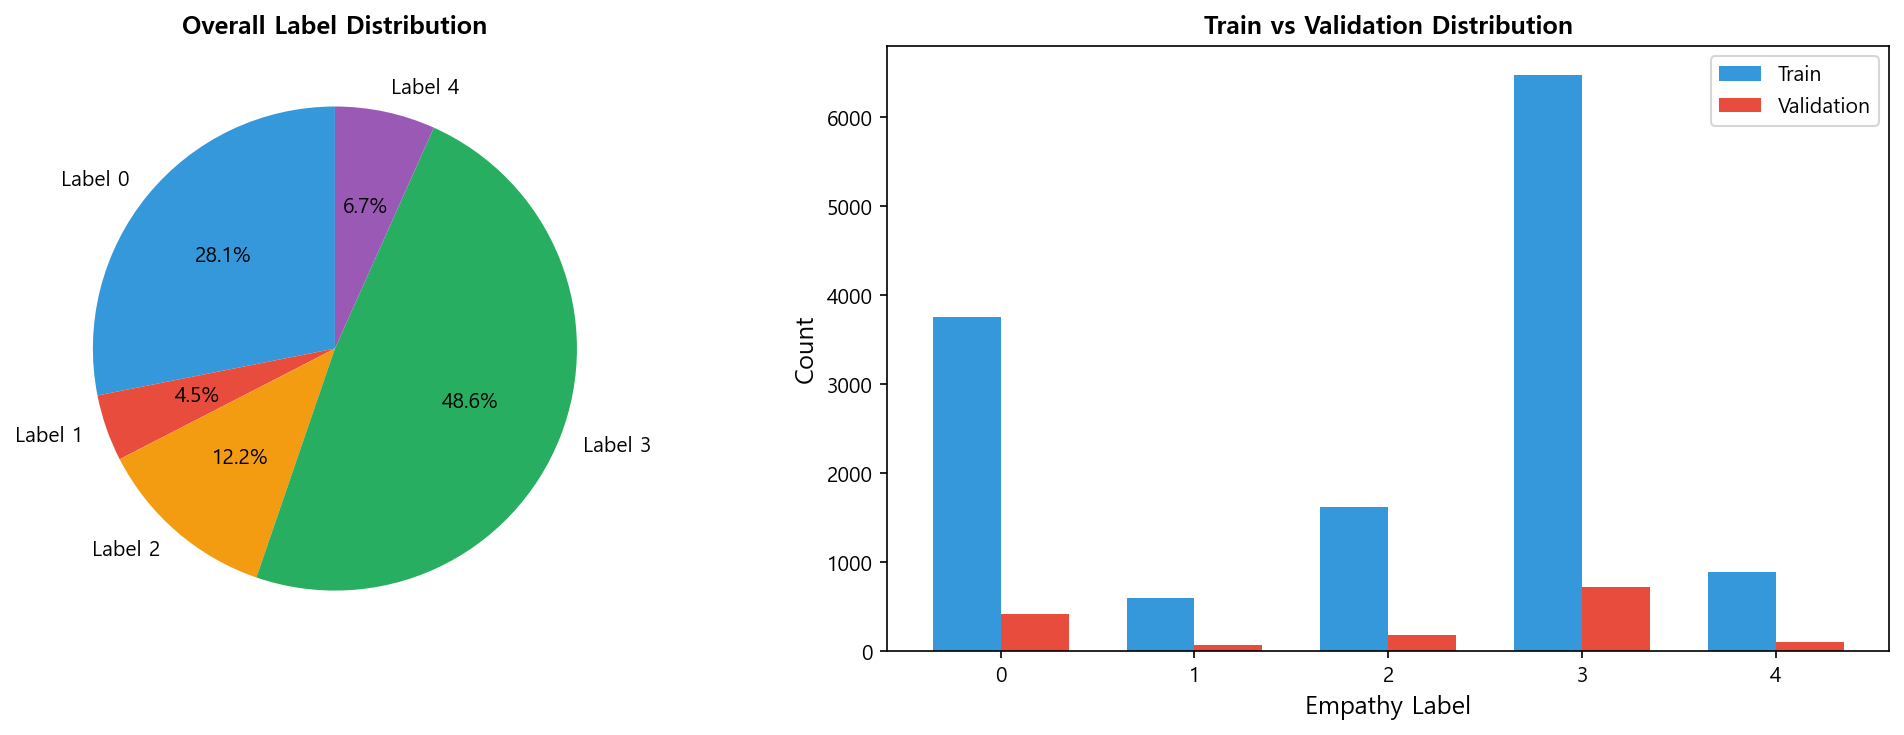
\includegraphics[width=0.95\textwidth]{figures/label_distribution.png}
    \caption{Empathy Label Distribution}
    \label{fig:label_dist}
    
    \vspace{0.5em}
    \footnotesize\textit{Note.} 왼쪽: 전체 데이터셋의 라벨 분포. 오른쪽: 학습(Train) 및 검증(Validation) 데이터셋의 라벨 분포 비교.
\end{figure}

\subsection{Train/Validation 분할}
데이터는 층화 샘플링(stratified sampling)을 통해 90:10 비율로 분할되었다.
각 라벨별 분포가 유지되도록 하였으며, 분할 결과는 Table~\ref{tab:train_val_split}에 제시되어 있다.

\begin{table}[H]
\centering
\caption{Train and Validation Set Label Distribution}
\label{tab:train_val_split}
\begin{tabular}{crrrr}
\toprule
\textbf{Label} & \textbf{Train} & \textbf{Train \%} & \textbf{Validation} & \textbf{Val \%} \\
\midrule
0 & 3,750 & 28.1\% & 417 & 28.1\% \\
1 & 594 & 4.5\% & 66 & 4.4\% \\
2 & 1,625 & 12.2\% & 181 & 12.2\% \\
3 & 6,478 & 48.6\% & 720 & 48.5\% \\
4 & 894 & 6.7\% & 100 & 6.7\% \\
\midrule
\textbf{Total} & \textbf{13,341} & \textbf{100.0\%} & \textbf{1,484} & \textbf{100.0\%} \\
\bottomrule
\end{tabular}

\vspace{0.5em}
\footnotesize\textit{Note.} 층화 샘플링을 통해 각 라벨의 비율이 Train과 Validation 세트에서 유사하게 유지되었다.
\end{table}

% ============================================
% 3. 방법론
% ============================================
\section{방법론}

\subsection{모델 구성}
본 연구에서는 OpenAI의 GPT-4.1 Nano 모델을 기반으로 fine-tuning을 수행하였다.
모델 구성 정보는 Table~\ref{tab:model_config}에 제시되어 있다.

\begin{table}[H]
\centering
\caption{Model Configuration}
\label{tab:model_config}
\begin{tabular}{ll}
\toprule
\textbf{Parameter} & \textbf{Value} \\
\midrule
Base Model & gpt-4.1-nano-2025-04-14 \\
Fine-tuned Model & ft:gpt-4.1-nano-2025-04-14:personal::Cn0GL0QT \\
Training Method & Supervised Fine-tuning (SFT) \\
Number of Epochs & 3 \\
Train/Val Split & 90\% / 10\% \\
Number of Classes & 5 (0, 1, 2, 3, 4) \\
\bottomrule
\end{tabular}

\vspace{0.5em}
\footnotesize\textit{Note.} Fine-tuning은 OpenAI API를 통해 수행되었다.
\end{table}

\subsection{프롬프트 설계}
모델 학습 및 추론에 사용된 프롬프트 구조는 다음과 같다:

\begin{Verbatim}[frame=single, fontsize=\small]
System: You are an empathy classifier for Korean persona-user 
        dialogues. Given a USER utterance and the PERSONA's 
        reply, output a JSON object ONLY with the key 
        "empathy_label" whose value is an integer in {0,1,2,3,4}.

User:   Classify the empathy level of the PERSONA's reply.
        USER: [user utterance]
        PERSONA: [persona response]
        Return JSON only.
\end{Verbatim}

\subsection{평가 지표}
모델 성능 평가를 위해 다음의 지표들을 사용하였다:
\begin{itemize}
    \item \textbf{Accuracy}: 전체 샘플 중 정확히 분류된 샘플의 비율
    \item \textbf{Macro Precision}: 각 클래스별 정밀도의 평균
    \item \textbf{Macro Recall}: 각 클래스별 재현율의 평균
    \item \textbf{Macro F1}: 각 클래스별 F1 점수의 평균
\end{itemize}

% ============================================
% 4. 텍스트 분석
% ============================================
\section{텍스트 분석}

\subsection{텍스트 길이 분포}
사용자와 페르소나의 발화 길이 분포는 Figure~\ref{fig:text_length}에 제시되어 있다.

\begin{figure}[H]
    \centering
    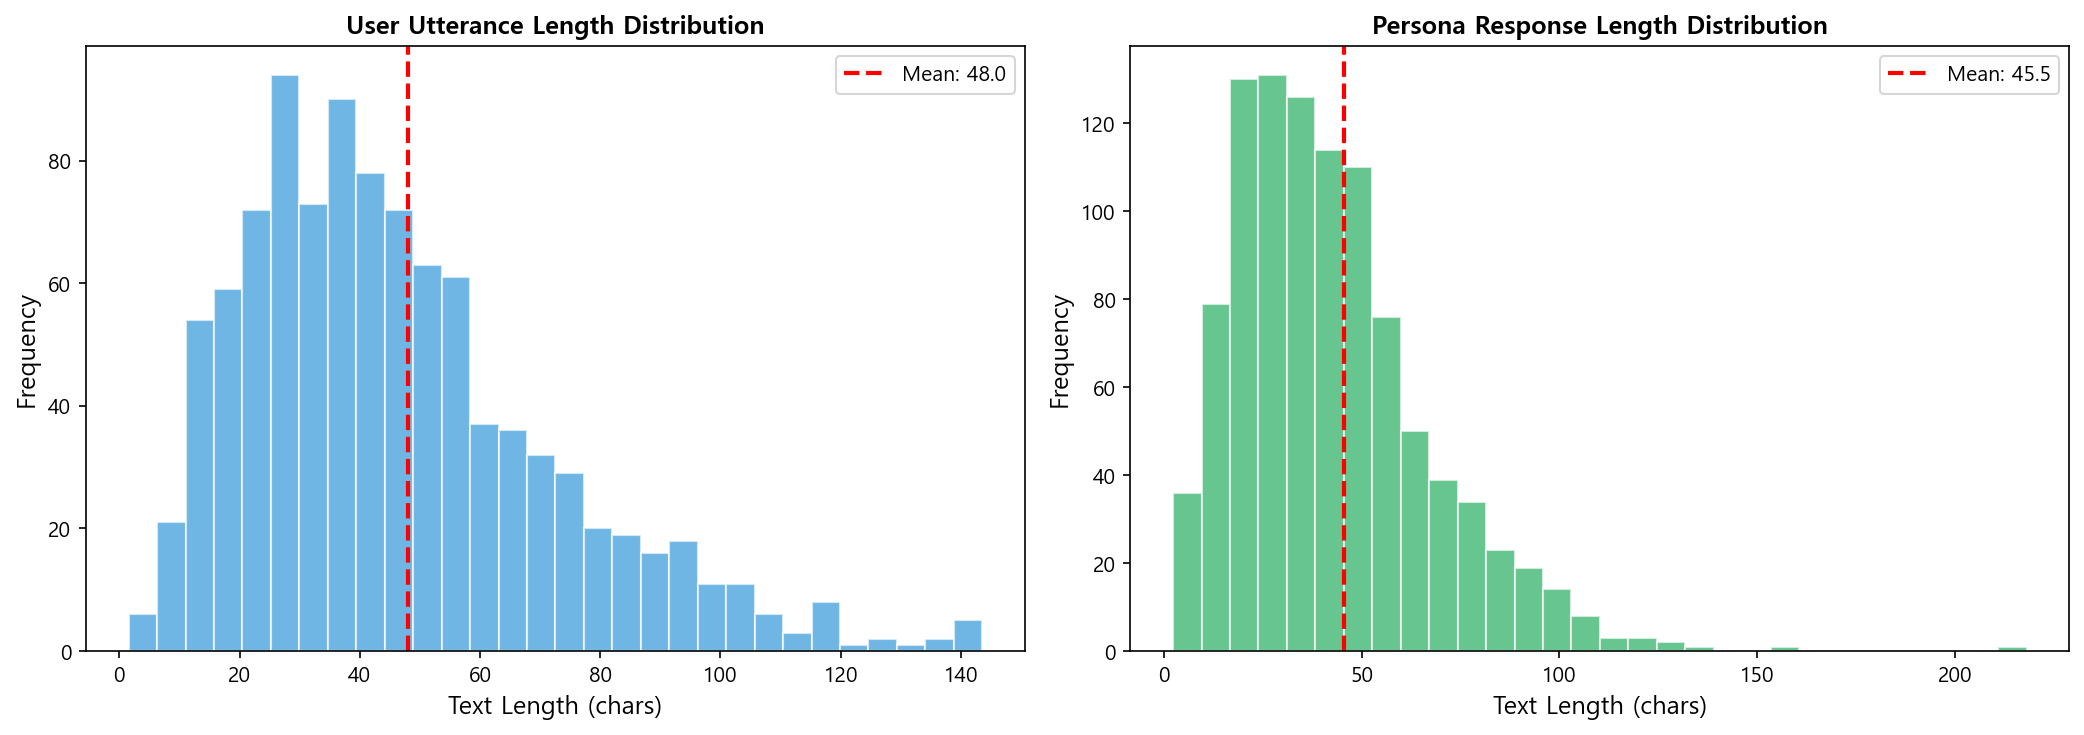
\includegraphics[width=0.95\textwidth]{figures/text_length.png}
    \caption{Text Length Distribution}
    \label{fig:text_length}
    
    \vspace{0.5em}
    \footnotesize\textit{Note.} 왼쪽: 사용자 발화 길이 분포. 오른쪽: 페르소나 응답 길이 분포. 빨간 점선은 평균값을 나타낸다.
\end{figure}

\subsection{공감 레벨별 응답 길이}
페르소나 응답 길이와 공감 레벨 간의 관계는 Figure~\ref{fig:boxplot}에 제시되어 있다.

\begin{figure}[H]
    \centering
    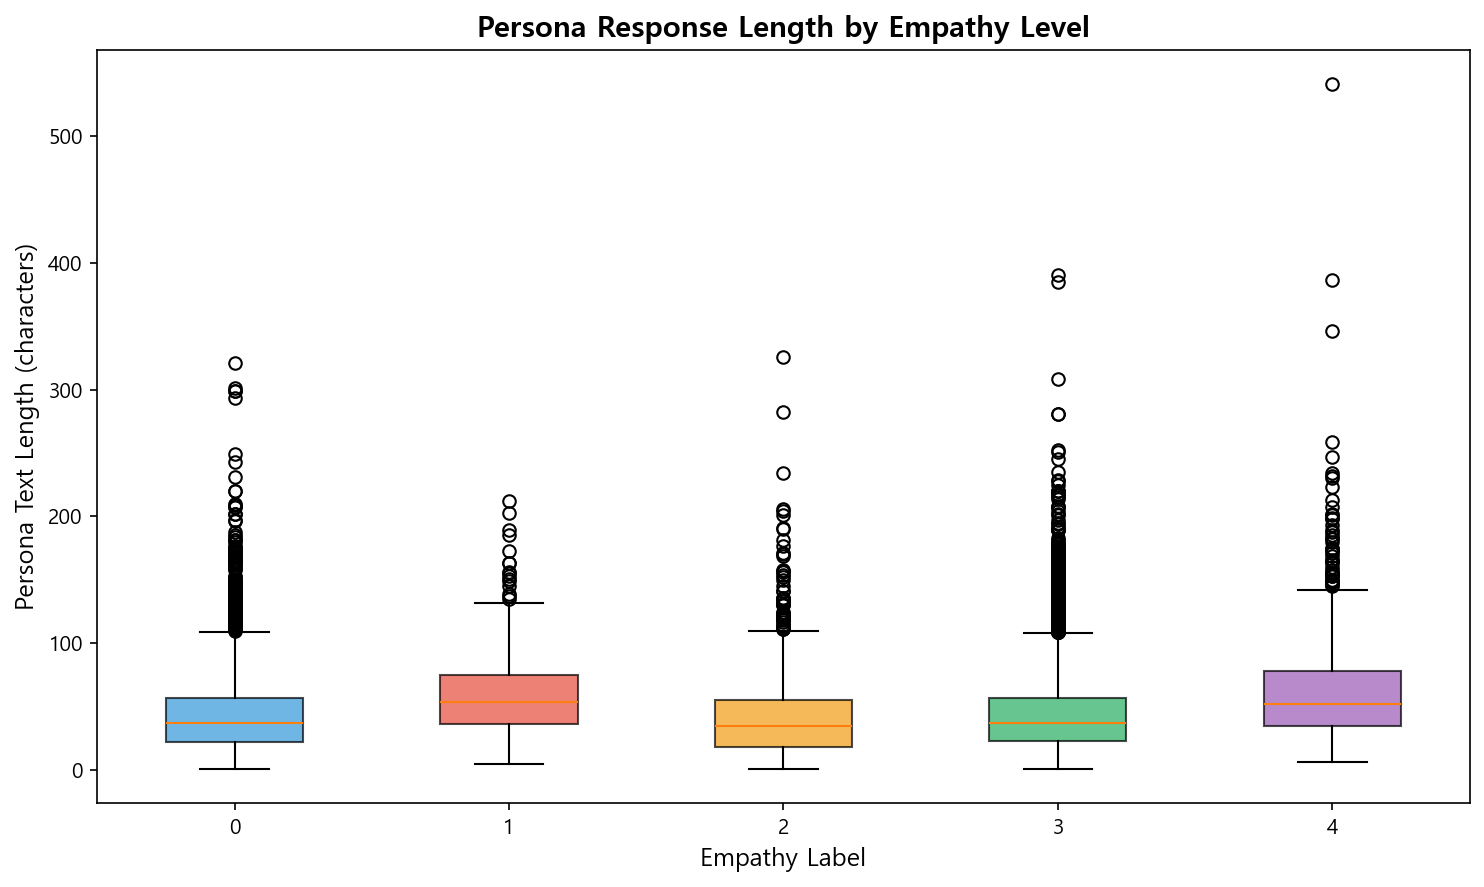
\includegraphics[width=0.8\textwidth]{figures/boxplot.png}
    \caption{Persona Response Length by Empathy Level}
    \label{fig:boxplot}
    
    \vspace{0.5em}
    \footnotesize\textit{Note.} 박스플롯은 각 공감 레벨별 페르소나 응답 길이의 분포를 나타낸다. 높은 공감 레벨에서 응답 길이가 더 긴 경향이 관찰된다.
\end{figure}

% ============================================
% 5. 분류 예시
% ============================================
\section{분류 예시}

Table~\ref{tab:examples}는 각 공감 레벨별 대표적인 대화 예시를 보여준다.

\begin{table}[H]
\centering
\caption{Example Dialogues for Each Empathy Level}
\label{tab:examples}
\begin{tabular}{cp{5cm}p{5cm}p{2cm}}
\toprule
\textbf{Level} & \textbf{User} & \textbf{Persona} & \textbf{Reason} \\
\midrule
0 & 안녕하세욤 & 안녕하세용!! & 단순 인사 \\
\midrule
1 & 앗.. 사실.. 나 아까 밖에 나갔다가 붕어빵 두 개 사서 하나 먹었어.. & 헉쓰!!! 승희야~붕어빵 칼로리 어마어마 한데!! & 비판에 초점 \\
\midrule
2 & 그러게 말이야 ㅎㅎ & 그러게..? & 최소한의 반응 \\
\midrule
3 & 정말!!! 파스타는 재료만 바꿔도 전혀 다른 요리로 바뀌는 점이 매력적이야! & 그렇지~ 아무래도 같은 재료로 여러 가지 도전할 수 있는 게 매력이야! & 적절한 동조 \\
\midrule
4 & 와....... 정말 꿀조합인걸 나 딸기빙수 환장하는데! & 헐 정말? 혹시 어디꺼? 난 설빙!!! & 적극적 관심 \\
\bottomrule
\end{tabular}

\vspace{0.5em}
\footnotesize\textit{Note.} 각 예시는 해당 공감 레벨의 특성을 잘 보여주는 대표적인 대화를 선정하였다.
\end{table}

% ============================================
% 6. 결론 및 향후 연구
% ============================================
\section{결론 및 향후 연구}

\subsection{결론}
본 프로젝트에서는 OPELA 데이터셋을 활용하여 한국어 대화에서 공감 수준을 자동으로 분류하는 
시스템을 개발하였다. 주요 성과는 다음과 같다:

\begin{itemize}
    \item OPELA 데이터셋(14,825 샘플)을 활용한 공감 분류 모델 구축
    \item GPT-4.1 Nano 모델의 효과적인 Fine-tuning
    \item 5단계 공감 레벨 자동 분류 시스템 개발
\end{itemize}

\subsection{향후 연구}
\begin{itemize}
    \item 더 큰 모델(GPT-4.1 Mini/Standard)로의 확장
    \item 멀티턴 컨텍스트를 반영한 학습
    \item 다양한 도메인 데이터 추가
    \item 다른 심리적 속성(self-disclosure, engaging 등) 분류기 개발
\end{itemize}

% ============================================
% 참고문헌
% ============================================
\section{참고문헌}

\begin{itemize}
    \item Smilegate AI \& Seoul National University (2022). OPELA: Open-domain conversations by Personas with Empathy, Long-term memory, and Attractive personality. GitHub: https://github.com/smilegate-ai/OPELA
    \item Lee, Y. K., Cho, W. I., Bae, S., Choi, H., Park, J., Kim, N. S., \& Hahn, S. (2022). "Feels like I've known you forever": empathy and self-awareness in human open-domain dialogs. PsyArXiv.
\end{itemize}

\end{document}
